%%%%%%%%%%%%%%%%%%%%%%%%%%%%%%%%%%%%%%%%%
% Programming/Coding Assignment
% LaTeX Template
%
% This template has been downloaded from:
% http://www.latextemplates.com
%
% Original author:
% Ted Pavlic (http://www.tedpavlic.com)
%
% Adapted by:
% Jacopo De Stefani (jacopo.de.stefani@gmail.com)
%
% Note:
% The \lipsum[#] commands throughout this template generate dummy text
% to fill the template out. These commands should all be removed when 
% writing assignment content.
%
% This template uses a Perl script as an example snippet of code, most other
% languages are also usable. Configure them in the "CODE INCLUSION 
% CONFIGURATION" section.
%
%%%%%%%%%%%%%%%%%%%%%%%%%%%%%%%%%%%%%%%%%

%----------------------------------------------------------------------------------------
%	PACKAGES AND OTHER DOCUMENT CONFIGURATIONS
%----------------------------------------------------------------------------------------

\documentclass{article}

\usepackage[utf8]{inputenc}
\usepackage{textcomp}
\usepackage{fancyhdr} % Required for custom headers
\usepackage{lastpage} % Required to determine the last page for the footer
\usepackage{extramarks} % Required for headers and footers
\usepackage[usenames,dvipsnames]{color} % Required for custom colors
\usepackage{graphicx} % Required to insert images
\usepackage{listings} % Required for insertion of code
\usepackage{courier} % Required for the courier font
\usepackage{lipsum} % Used for inserting dummy 'Lorem ipsum' text into the template
\usepackage{rotating}
\usepackage{natbib}
\usepackage{graphicx}
\usepackage{tikz}
\usepackage{pgfplots}
\usepackage{multicol}
\usepackage{caption}
\usepackage{amsmath}
\usepackage{amsfonts}
\usepackage{algpseudocode}% http://ctan.org/pkg/algorithmicx
\usepackage{algorithm}% http://ctan.org/pkg/algorithm
\usepackage{pdflscape}
\usepackage{hyperref}
\usepackage{pifont}
\usepackage{subcaption}

\usetikzlibrary{positioning,shadows,arrows,intersections,calc,automata}

% Margins
\topmargin=-0.45in
\evensidemargin=0in
\oddsidemargin=0in
\textwidth=6.5in
\textheight=9.0in
\headsep=0.25in

\linespread{1.1} % Line spacing

% Set up the header and footer
\pagestyle{fancy}
\lhead{} % Top left header
\chead{\hmwkClass\ (\hmwkClassInstructor) : \hmwkTitle} % Top center head
\rhead{}%\firstxmark} % Top right header
\lfoot{\hmwkAuthorName} % Bottom left footer
\cfoot{}%\lastxmark} % Bottom center footer
\rfoot{Page\ \thepage\ of\ \protect\pageref{LastPage}} % Bottom right footer
\renewcommand\headrulewidth{0.4pt} % Size of the header rule
\renewcommand\footrulewidth{0.4pt} % Size of the footer rule

\setlength\parindent{0pt} % Removes all indentation from paragraphs

%----------------------------------------------------------------------------------------
%	CODE INCLUSION CONFIGURATION
%----------------------------------------------------------------------------------------

\definecolor{MyDarkGreen}{rgb}{0.0,0.4,0.0} % This is the color used for comments
\lstloadlanguages{Python} % Load Perl syntax for listings, for a list of other languages supported see: ftp://ftp.tex.ac.uk/tex-archive/macros/latex/contrib/listings/listings.pdf
\lstset{language=Python, % Use Perl in this example
        frame=single, % Single frame around code
        basicstyle=\small\ttfamily, % Use small true type font
        keywordstyle=[1]\color{Blue}\bf, % Perl functions bold and blue
        keywordstyle=[2]\color{Purple}, % Perl function arguments purple
        keywordstyle=[3]\color{Blue}\underbar, % Custom functions underlined and blue
        identifierstyle=, % Nothing special about identifiers                                         
        commentstyle=\usefont{T1}{pcr}{m}{sl}\color{MyDarkGreen}\small, % Comments small dark green courier font
        stringstyle=\color{Purple}, % Strings are purple
        showstringspaces=false, % Don't put marks in string spaces
        tabsize=5, % 5 spaces per tab
        %
        % Put standard Perl functions not included in the default language here
        morekeywords={rand},
        %
        % Put Perl function parameters here
        morekeywords=[2]{on, off, interp},
        %
        % Put user defined functions here
        morekeywords=[3]{test},
       	%
        morecomment=[l][\color{Blue}]{...}, % Line continuation (...) like blue comment
        numbers=left, % Line numbers on left
        firstnumber=1, % Line numbers start with line 1
        numberstyle=\tiny\color{Blue}, % Line numbers are blue and small
        stepnumber=5, % Line numbers go in steps of 5
        breaklines=true
}

% Creates a new command to include a perl script, the first parameter is the filename of the script (without .pl), the second parameter is the caption
\newcommand{\pyscript}[2]{
\begin{itemize}
\item[]\lstinputlisting[caption=#2,label=#1]{#1.py}
\end{itemize}
}

%----------------------------------------------------------------------------------------
%	DOCUMENT STRUCTURE COMMANDS
%	Skip this unless you know what you're doing
%----------------------------------------------------------------------------------------

% Header and footer for when a page split occurs within a problem environment
\newcommand{\enterProblemHeader}[1]{
\nobreak\extramarks{#1}{#1 continued on next page\ldots}\nobreak
\nobreak\extramarks{#1 (continued)}{#1 continued on next page\ldots}\nobreak
}

% Header and footer for when a page split occurs between problem environments
\newcommand{\exitProblemHeader}[1]{
\nobreak\extramarks{#1 (continued)}{#1 continued on next page\ldots}\nobreak
\nobreak\extramarks{#1}{}\nobreak
}

\setcounter{secnumdepth}{0} % Removes default section numbers
\newcounter{homeworkProblemCounter} % Creates a counter to keep track of the number of problems

\newcommand{\homeworkProblemName}{}
\newenvironment{homeworkProblem}[1][Problem \arabic{homeworkProblemCounter}]{ % Makes a new environment called homeworkProblem which takes 1 argument (custom name) but the default is "Problem #"
\stepcounter{homeworkProblemCounter} % Increase counter for number of problems
\renewcommand{\homeworkProblemName}{#1} % Assign \homeworkProblemName the name of the problem
\section{\homeworkProblemName} % Make a section in the document with the custom problem count
\enterProblemHeader{\homeworkProblemName} % Header and footer within the environment
}{
\exitProblemHeader{\homeworkProblemName} % Header and footer after the environment
}

\newcommand{\problemAnswer}[1]{ % Defines the problem answer command with the content as the only argument
\noindent\framebox[\columnwidth][c]{\begin{minipage}{0.98\columnwidth}#1\end{minipage}} % Makes the box around the problem answer and puts the content inside
}

\newcommand{\homeworkSectionName}{}
\newenvironment{homeworkSection}[1]{ % New environment for sections within homework problems, takes 1 argument - the name of the section
\renewcommand{\homeworkSectionName}{#1} % Assign \homeworkSectionName to the name of the section from the environment argument
\subsection{\homeworkSectionName} % Make a subsection with the custom name of the subsection
\enterProblemHeader{\homeworkProblemName\ [\homeworkSectionName]} % Header and footer within the environment
}{
\enterProblemHeader{\homeworkProblemName} % Header and footer after the environment
}

%----------------------------------------------------------------------------------------
%	USER DEFINED TIKZ STYLES
%----------------------------------------------------------------------------------------

\tikzset{
    player1/.style={circle, draw=none, fill=green!70!black, circular drop shadow,
        text centered, anchor=north, text=white},
    player2/.style={circle, draw=none, fill=orange, circular drop shadow,
        text centered, anchor=north, text=white},
    chance/.style={circle, draw,text centered, anchor=north},
    subtreeB/.style={rectangle, draw, rounded corners=1mm, color=red, thick,
        text centered, anchor=north, text=red},
    subtreeC/.style={rectangle, draw, rounded corners=1mm, color=orange, thick,
        text centered, anchor=north, text=orange},
    ex2/.style={circle, draw,text centered, anchor=north},
    nashEq1P/.style={circle,draw=none, fill=green!70!black, text centered, anchor=north, text=white,inner sep=2pt},
    nashEq2P/.style={circle,draw=none, fill=orange, text centered, anchor=north, text=white,inner sep=2pt},
    nashEqPoints/.style={fill=white,draw=black,thick},
    level distance=0.5cm, growth parent anchor=south
}

\tikzstyle{tier}=[draw, fill=yellow!20, text width=6.0em, text centered,
  minimum height=1.5em,drop shadow]
\tikzstyle{component} = [tier, text width=8em, minimum width=10em,
  minimum height=3em, rounded corners, drop shadow,inner sep=2pt]
\tikzstyle{texto} = [above, text width=6em, text centered]
\tikzstyle{linepart} = [draw, thick, color=black!50, -latex', dashed]
\tikzstyle{line} = [draw, thick, color=black!50, -latex', ->]
\tikzstyle{ur}=[draw, text centered, minimum height=0.01em]
 
% Define distances for bordering
\newcommand{\blockdist}{1.3}
\newcommand{\edgedist}{1.5}

\newcommand{\component}[2]{node (p#1) [component]
  {{\scriptsize\textit{#2}}}}


% Draw background
\newcommand{\backgroundSquare}[5]{%
  \begin{pgfonlayer}{background}
    % Left-top corner of the background rectangle
    \path (#1.west |- #2.north)+(-0.5,0.5) node (a1) {};
    % Right-bottom corner of the background rectanle
    \path (#3.east |- #4.south)+(+0.5,-0.25) node (a2) {};
    % Draw the background
    \path[fill=blue!20,rounded corners, draw=black!50, dashed]
      (a1) rectangle (a2);
    \path (a1.east |- a1.south)+(0.8,-0.3) node (u1)[texto]
      {\scriptsize\textit{#5 Tier}};
  \end{pgfonlayer}}


\newcommand*\circled[2]{\tikz[baseline=(char.base)]{
            \node[#2,rectangle, rounded corners=0.7mm, text=white] (char) {#1};}}
\newcommand*\cellvcenter[1]{\raisebox{-\height}{#1}}


\newcommand{\cmark}{\ding{51}}%
\newcommand{\xmark}{\ding{55}}%
\newcommand{\HRule}{\rule{\linewidth}{0.5mm}}%

%----------------------------------------------------------------------------------------
%	NAME AND CLASS SECTION
%----------------------------------------------------------------------------------------

\newcommand{\hmwkTitle}{Swarm Robotics Project - Chaining Strategy} % Assignment title
\newcommand{\hmwkDueDate}{Wednesday,\ April\ 10,\ 2013} % Due date
\newcommand{\hmwkClass}{INFO-H-414 - Swarm Intelligence} % Course/class
\newcommand{\hmwkClassTime}{} % Class/lecture time
\newcommand{\hmwkClassInstructor}{Prof. M. Dorigo} % Teacher/lecturer
\newcommand{\hmwkAuthorName}{Jacopo De Stefani} % Your name
\newcommand{\maxmin}{$\mathcal{MAX}-\mathcal{MIN}$}

%----------------------------------------------------------------------------------------
%	TITLE PAGE
%----------------------------------------------------------------------------------------

\title{
\vspace{2in}
\textmd{\textbf{\hmwkClass:\\ The Traveling Salesman Problem with Time Windows \\ Stochastic Local Search Algorithms}}\\
%\normalsize\vspace{0.1in}\small{Due\ on\ \hmwkDueDate}\\
\vspace{0.1in}\large{\textit{\hmwkClassInstructor\ }}
\vspace{3in}
}

\author{\textbf{\hmwkAuthorName}}
\date{\today} % Insert date here if you want it to appear below your name

%----------------------------------------------------------------------------------------

\begin{document}

\begin{titlepage}

\begin{center}


% Upper part of the page

\includegraphics[width=0.70\textwidth]{./Figures/logo-ulb}\\[1cm]    

\textsc{\LARGE Université Libre de Bruxelles}\\[1.5cm]

\textsc{\Large INFO-H-414 - Swarm Intelligence}\\[0.5cm]


% Title
\HRule \\[0.4cm]
{ \huge \bfseries Swarm Robotics Project: \\ Chain Formation Strategy}\\[0.4cm]

\HRule \\[1cm]

% Author and supervisor
\begin{minipage}{0.4\textwidth}
\begin{flushleft} \large
\emph{Author:}\\
Jacopo  \textsc{De Stefani}
\end{flushleft}
\end{minipage}
\begin{minipage}{0.4\textwidth}
\begin{flushright} \large
\emph{Supervisors:} \\
Prof.~Marco \textsc{Dorigo}\\
Prof.~Mauro \textsc{Birattari}
\end{flushright}
\end{minipage}

\vfill

% Bottom of the page
{\large \today}

\end{center}

\end{titlepage}

%\maketitle

%----------------------------------------------------------------------------------------
%	TABLE OF CONTENTS
%----------------------------------------------------------------------------------------

%\setcounter{tocdepth}{1} % Uncomment this line if you don't want subsections listed in the ToC

\newpage
\tableofcontents
\newpage
 
\section{Controller overview}
\subsection{General structure}
The robot controller has been structured according to the sense-think-act paradigm.

In fact, at each time step, the robots will:
\begin{enumerate}
  \item \emph{(Sense)} - Read the informations collected by the available sensors.
  \item \emph{(Think)} - Determine the values to send to the actuators according to the state machine defined in \nameref{sec:sm} and the information from the sensors.
  \item \emph{(Act)} - Control the actuators.
\end{enumerate}

In terms of code:
\begin{enumerate}
  \item \emph{(Sense)} - The \emph{ParseX} function are used to read the values of the different sensors (proximity, ground, distance scanner and Range and Bearing) and provide information to the following step in a suitable form (e.g. repulsion vector or beacon table).
  \item \emph{(Think)} - The core of the behavior is implemented as a finite state machine (FSM), where each state is implemented as function.
  In this way the controller of the robot just need to execute the function corresponding to the agent's current state.
  \item \emph{(Act)} - According to the position, and the control values computed in the previous step, determine the speeds to actuate on the wheels and the information to broadcast using 
  the Range and Bearing System.
\end{enumerate}

\subsection{Potential field approach}
Researchers in Swarm Robotics try to understand how a behavior at the swarm level could emerge from local interactions at the robot level, using information either coming from the environment or from other robots.

Among the different models of these interactions that can be found in the literature, I decided to apply the potential-field approach (cf.\cite{howard2002mobile}), based on the readings from the sensors.

These virtual potential fields $U_i$ are defined on the whole environment and robots are able to compute locally the force $\mathbf{F}_i$ resulting from the interaction with the corresponding field as:
\begin{equation}
  \mathbf{F}_i = -\nabla U_i
\end{equation}
With this approach, it is possible to explicitly construct a field $U_i$ to induce a certain behavior on the robot.
For this purpose, the following virtual fields have been defined:
\begin{itemize}
  \item Obstacle avoidance - $U_{obs}$
  \item Distance scanner - $U_{ds}$
  \item Range and Bearing - $U_{rab}$
\end{itemize} 

The resulting forces from the aforementioned vector fields are determined from the corresponding sensor readings.
That is, each reading is transformed into a vector whose angle and magnitude depends on the value of the reading itself.
All the vector are expressed in polar coordinates, in the form ($\rho$\emph{(Magnitude)},$\alpha$\emph{(Angle)}).
Note that $\mathbf{F_{obs}}$ and $\mathbf{F_{obs}}$ are repulsive, while $\mathbf{F_{rab}}$ 
is attractive.

\paragraph{Obstacle avoidance}
\begin{equation}
\mathbf{p_i} = (r_{prox_{i}},\theta_i)  
\end{equation}
where $r_{prox_i}$ corresponds to the value of the reading of the $i^{th}$ proximity sensor and $\theta_i$ is the corresponding angle.

\begin{align}
 \mathbf{F_{obs}} = (1.5,\theta_{sp}) & & \mathbf{sp} = \sum_i -\mathbf{p_i}  
\end{align}
where $\theta_{sp}$ corresponds to the angle of $\mathbf{sp}$ vector.

\paragraph{Distance scanner}
\begin{equation}
\mathbf{ds_i} = (1 - \frac{150 - r_{ds_{i}}}{150-4},\theta_i)  
\end{equation}
where $r_{prox_i}$ corresponds to the value of the $i^{th}$ reading of the distance and $\theta_i$ is the corresponding angle.
The value of the distance scanner reading is normalized in the range $(4[cm],150[cm])$ 
i.e. (\emph{Lower bound short range readings}, \emph{Upper bound long range readings}).
By subtracting the normalized value to 1, one is able to obtain a vector whose 
magnitude is increases linearly as the distance from the obstacle decrease.

\begin{align}
\mathbf{F_{ds}} = (1.0,\theta_{sds}) & & \mathbf{sds} = \sum_i -\mathbf{ds_i} 
\end{align}
where $\theta_{sds}$ corresponds to the angle of $\mathbf{sds}$ vector.

\paragraph{Range and Bearing}
\begin{equation}
\mathbf{F_{rab}} = (1.0,\theta_{rab})  
\end{equation}
where $\theta_{rab}$ corresponds to the angle of RAB reading.

\subsection{General idea}
The general idea of the method is that the robots should first quit the initial deployment room, characterized by four surrounding walls, one of them containing an opening to let the robots move outside, and a dark grey floor, to then start the exploration phase required to find the target spots.

In order to reduce the interference phenomenon at the exit of the nest, a sequential deployment mechanism based on the robot id has been developed.

After exiting the nest, the agents should explore the environment, either individually (as \emph{explorers}) or using the collectivly-gathered knowledge of the environment (i.e. the chain).

If no information is available, the robot could decide (stochastically) to become a starting point for a new chain in the environment.

Otherwise, the exploration of the environment should, in principle, profit of the already available knowledge.

Nevertheless, this method achieves the required chain formation behavior using the embodied information in the chain only to exist the nest, while the successive exploration is simply guided by proximity sensors and the distance scanner.
 

\paragraph{Rules}\label{par:rules}
The actual chain formation behavior is driven by five simple rules:
\begin{enumerate}
  \item If the \textbf{nest} has been \textbf{left}, and \textbf{no} chain beacon have been already \textbf{sensed}, after $t_{ns}$ time step, decide with probability $p_{btoe}$ to stop and become a chain end.
  \item If the \textbf{nest} has been \textbf{left}, and \textbf{exactly one} chain beacon has been \textbf{sensed} at a distance greater than $d_{chain}$, stop and become a chain end.
  \item If a \textbf{chain end} has \textbf{more than one} neighboring\textbf{ beacon}, but \textbf{less than three}, then it changes its state to \emph{Chain member}.
  \item If a \textbf{chain member} has \textbf{more than two} neighboring \textbf{beacons}, then it changes its state to \emph{Chain junction}.
  \item The chain identifier of a new beacon is determined by incrementing of one unit the chain id of the closest beacon.
\end{enumerate}

\paragraph{Chain structure}
The chain will then be composed by three different kind of robots:
\begin{itemize}
  \item \textbf{(E) - Chain end:} Any robot connected to at most one other agent.
  \item \textbf{(M) - Chain member:} Any robot connected to exactly two agents.
  \item \textbf{(J) - Chain junction:} Any robot connected to more than two agents.
\end{itemize}

\begin{center}
\begin{tikzpicture}[shorten >=1pt,node distance=3cm,on grid,auto] 
   \node[state,accepting] (R1)   {$E_0$}; 
   \node[state,thick] (R2) [right=of R1] {$M_1$};
   \node[state,thick] (R3) [right=of R2] {$J_2$};
   \node[state,accepting,thick] (R4) [above right=of R3] {$E_3$};
   \node[state,thick] (R5) [below right=of R3] {$M_3$};
   \node[state,accepting,thick] (R6) [right=of R5] {$E_4$};
    \path[]
    (R1) edge (R2)
    (R2) edge (R3)
    (R3) edge (R4)
    (R3) edge (R5)
    (R5) edge (R6);
\end{tikzpicture}
\captionof{figure}{Chain example with nodes labeling and id}
\end{center}

\subsection{References}

Concerning the chain formation rules, the main sources of inspiration were \cite{nouyan2004chain}, \cite{nouyan2008path} which helped me to better understand the chain structure (in particular, how to distinguish elements in the chain) and the chain navigation behavior (which have not been implemented here) and \cite{goss1992harvesting} for defining the conditions to extend the chain.

Furthermore, the idea of an incremental deployment has been taken from \cite{stirling2013energy}.

While in \cite{stirling2013energy} the incremental deployment was used to limit energy consumption in the deployment phase, here the same idea is used to prevent the interference phenomenon that could occur at the nest exit.

In fact, whenever a relevant number of robots (10+) tries to exit the nest at the same time, each agent will spend more time performing obstacle avoidance with respect to one another, rather than actually exiting the nest.


%\begin{equation}
  %\text{Ticks per complete revolution} = \frac{\pi [rad]}{\omega [\frac{rad}{s}]} \cdot tps [\frac{tick}{s}]
%\end{equation}


% \subsubsection{Logical FSM}

% \begin{center}
% \begin{tikzpicture}[shorten >=1pt,node distance=5cm,on grid,auto] 
%    \node[state,initial] (Ex)   {Exploration}; 
%    \node[state] (As) [below right=of Ex] {Assessing cluster}; 
%    \node[state] (Uw) [below left=of Ex] {Unit work};
%    \node[state] (De) [below left=of As] {Decision phase};
%     \path[->] 
%     (Ex) edge [bend left]  node  {Sense light} (As)
%     (As) edge [bend left]  node  {In sensing range} (De)
%     (De) edge node [right]  {Full cluster} (Ex) 
%         edge [bend left] node {Empty stations} (Uw)
%     (Uw) edge [bend left]  node [above right]  {End work} (De) ;
% \end{tikzpicture}
% \captionof{figure}{Logical FSM for the E-puck behavior}
% \end{center}

% \subsubsection{Real FSM}

 

% \subsection{TAM}
% The task are represented by spatially distributed booths.

% The robots must reach and enter the booth to undertake the corresponding working activity.


% \subsubsection{Logical FSM}

% \begin{center}
% \begin{tikzpicture}[shorten >=1pt,node distance=3cm,on grid,auto] 
%    \node[state,initial,thick,draw=green!75,fill=green!20,] (Av)   {Available}; 
%    \node[state,thick,draw=red!75,fill=red!20] (Oc) [below right=of Av] {Occupied}; 
%    \node[state,thick,draw=yellow!75,fill=yellow!20] (Un) [below left=of Av] {Unavailable};
%     \path[->] 
%     (Av) edge [bend left]  node  {Sense Robot} (Oc)
%     (Oc) edge [bend left]  node  {$T_w$ expired} (Un)
%     (Un) edge [bend left] node [left]  {Robot not sensed} (Av);
% \end{tikzpicture}
% \captionof{figure}{Logical and Implemented FSM for the TAM behavior}
% \end{center}

\section{Controller details} \label{sec:sm}

\begin{center}
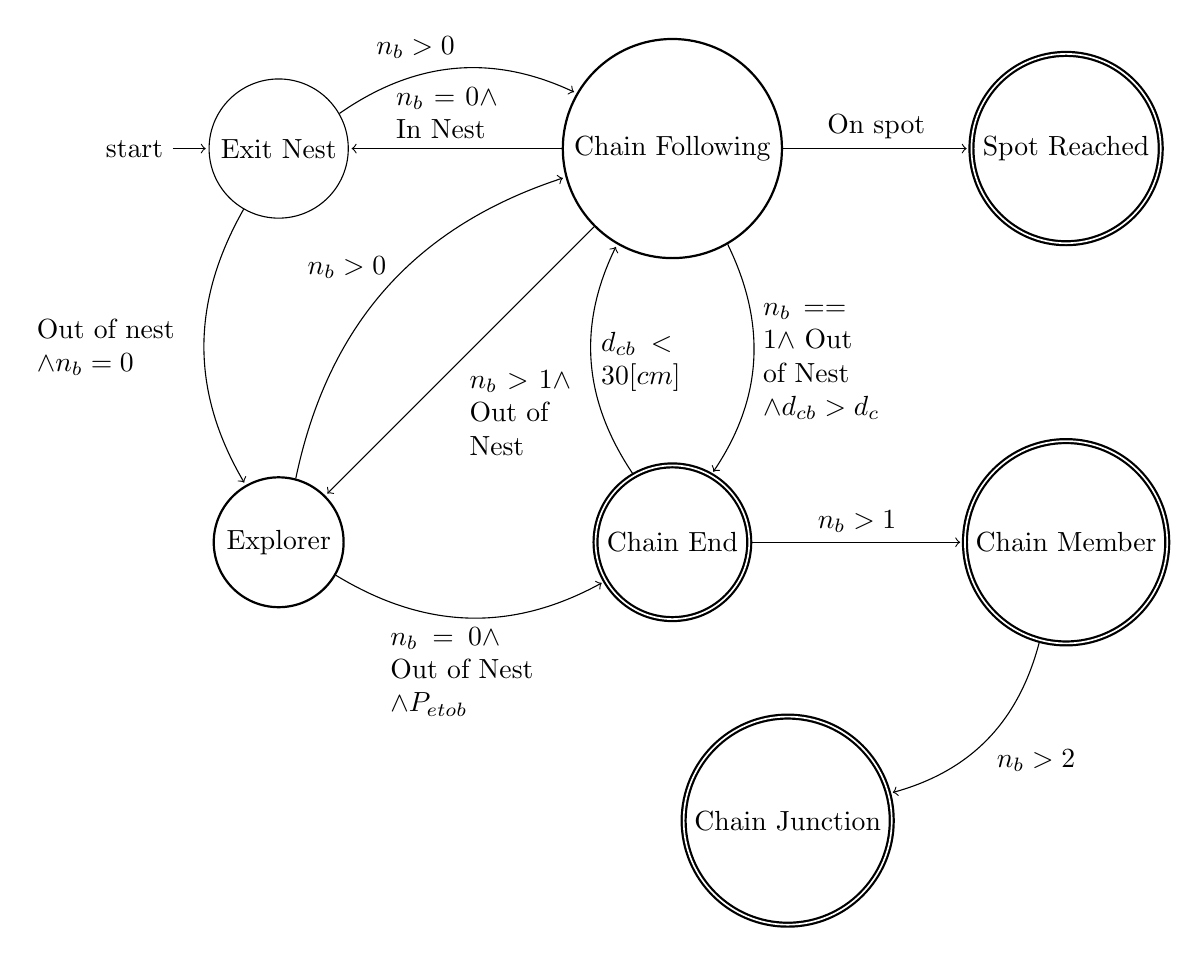
\begin{tikzpicture}[shorten >=1pt,node distance=5cm,on grid,auto] 
   \node[state,initial] (EN)   {Exit Nest}; 
   \node[state,thick] (EX) [below=of EN] {Explorer};
   \node[state,thick] (EC) [right=of EN] {Chain Following};
   \node[state,accepting,thick] (SR) [right=of EC] {Spot Reached};
   \node[state,accepting,thick] (CE) [below =of EC] {Chain End};
   \node[state,accepting,thick] (CM) [right=of CE] {Chain Member};
   \node[state,accepting,thick] (CJ) [below left=of CM] {Chain Junction};
    \path[->] 
    (EN) edge [bend right]  node [left,text width=2cm]  {Out of nest $\wedge \text{} n_b = 0$} (EX)
         edge [bend left]  node [above,text width=2cm]  {$n_b >0$} (EC)
    (EX) edge [bend left]  node [above,text width=2cm]  {$n_b >0$} (EC)
         edge [bend right]  node [below,text width=2cm]  {$n_b = 0 \text{} \wedge$ Out of Nest $\wedge \text{} P_{etob}$} (CE)
    (CE) edge node  {$n_b > 1$} (CM)
           edge [bend left] node [right,text width=1.5cm]  {$d_{cb} < 30[cm]$} (EC)
    (CM) edge [bend left] node [text width=2cm] {$n_b > 2$} (CJ)
    (EC) edge  node [above,text width=1.5cm]  {$n_b = 0 \text{} \wedge$ In Nest} (EN)
           edge  node [text width=1.5cm]  {$n_b > 1 \text{} \wedge$ Out of Nest} (EX) 
           edge [bend left] node [right,text width=1.5cm] {$n_b == 1 \text{} \wedge$ Out of Nest $\wedge \text{} d_{cb} > d_c$} (CE)
           edge  node {On spot} (SR);
\end{tikzpicture}
\captionof{figure}{Implemented FSM for the \emph{s-bot} chain formation behavior}
\end{center}

\paragraph{Controller parameters}
\begin{center}
\begin{tabular}{|c|c|c|}
\hline
\textbf{Parameter} & \textbf{Description} & \textbf{Value} \\ \hline
$v_{wheel}$ & Wheel velocity (straight movement) & $10 [\frac{cm}{s}]$ \\ \hline
$P_{etob}$ & Probability of starting a chain while being an explorer & 0.05 \\ \hline
$d_{chain}$ & Minimum distance among elements in the chain  & 130 [cm] \\ \hline
$\omega_{ds}$ & Angular rotation velocity of the distance sensor & $2\pi [\frac{rad}{s}]$ \\ \hline
$t_{ns}$ & Delay time on the decision to stop outside the nest & 100 [steps] \\ \hline
\end{tabular}
\captionof{table}{Controller parameters overview}
\label{tab:parameters}
\end{center}

\subsection{Resulting forces}

\subsection{States details}
\paragraph{Exit nest} \label{par:exitnest}
\begin{equation}
  \mathbf{F_{res}} = \mathbf{F_{obs}} + \mathbf{F_{ds}} + \mathbf{F_{rab}}
\end{equation}

The exit nest state is the initial state of the robots, which is maintained as long as it remains in the nest.
The robots uses the distance scanner and proximity sensors to find their way out 
of the nest.
In addition to those forces, the robot is also attracted (by means of $\mathbf{F_{rab}}$) 
towards the closest robots in the RAB sensing range that are in the \emph{Explorer} 
or the \emph{Chain following} state.
This is done beacause such kind of robots are either directing or already 
outside of the nest, thus following them will guide a robot in the right 
direction.
If a robots senses any kind of beacon it changes its state to \emph{Chain following}
Otherwise, it passes in \emph{Explorer} state.

\paragraph{Explorer}
\begin{equation}
  \mathbf{F_{res}} = \mathbf{F_{obs}} + \mathbf{F_{ds}} + \mathbf{F_{str}}
\end{equation}
In the \emph{Explorer} state, if no beacon is sensed, the robot moves outsides the nest without making any decision for $t_{ns}$ time steps, then deciding, at each simulation step, whether to stop or not.

The decision is stochastic and occurs with probability $P_{etob}$.

Otherwise, the robot goes straight ($\mathbf{F_{str}} = (1.0,0)$).

In any case, if the agent goes back to the nest, it enters the \emph{Exit Nest} state.

\paragraph{Chain following} \label{par:chainfollowing}
\begin{equation}
  \mathbf{F_{res}} = \mathbf{F_{obs}} + \mathbf{F_{ds}} + \mathbf{F_{str}}
\end{equation}
The \emph{Chain Following} state simply consists of a random walk of the robot 
in the environment.

The robots normally goes straight (guided by $\mathbf{F_{str}} = (1.0,0)$).

Its direction is then modified by the perceived obstacles both in a short range ($\mathbf{F_{obs}}$) and in a long range 
($\mathbf{F_{ds}}$).

As soon as the distance of a robot from the closest beacon is greater than the minimum chain distance ($d_{cb} > d_c$)
and exactly one beacon is sensed nearby ($n_b == 1$) (cfr. \nameref{par:rules} (2)) 
the robots stops and becomes a \emph{Chain End}.

If the robot loses contact with a chain beacon, it turns itself of 180 degrees. before 
restarting exploration.

In any case, if the agent goes back to the nest, it enters the \emph{Exit Nest} state.


\paragraph{Chain End}
\begin{equation}
  \mathbf{F_{res}} = (0,0)
\end{equation}
The \emph{Chain End} state is reached when a robot connects himself to the current end of the chain, becoming thus the new termination.

In this state, the robot stands still and broadcast information concerning its state, id and chain\_id to the neighboring robots.

If any beacon is sensed within 30 cm the robot starts moving again, in order to 
find a better position where to attach in the chain.

The transition to the \emph{Chain Member} state occurs anytime another agent connects to the current one.

\paragraph{Chain Member}
\begin{equation}
  \mathbf{F_{res}} = (0,0)
\end{equation}
A \emph{Chain Member} only acts as a beacon, broadcasting state information and acting as a relay for the back-propagation of the \emph{Target found} message.
A \emph{Chain Member} robot becomes a \emph{Chain Junction} if another robot decides to 
join the chain by attaching to it.

\paragraph{Chain Junction}
\begin{equation}
  \mathbf{F_{res}} = (0,0)
\end{equation}
The sole purpose of a \emph{Chain Junction} is to differentiate himself from the other beacons and stop the back-propagation of the \emph{Target found} message.

\section{Results} \label{sec:results}

\begin{center}
\begin{tabular}{|c|c|c|}
\hline
\textbf{Parameter} & \textbf{Description} & \textbf{Value} \\ \hline
$n_r$ & Number of \emph{s-bots} & $50$ \\ \hline
$r_{rab}$ & Range and Bearning Range & $150$ [cm] \\ \hline
$n_s$ & Number of simulations & $50$ \\ \hline
$seed$ & Seed value for the simulation & \verb|$RANDOM|\footnotemark[1] \\ \hline
$tps$ & Simulation steps per second & 10 \\ \hline
\end{tabular}
\captionof{table}{Simulation parameters overview}
\label{tab:simparameters}
\end{center}
\footnotetext[1]{Internal function of the Bash shell. \url{http://tldp.org/LDP/abs/html/randomvar.html}}

\subsection{Metric definitions}\label{subsec:metric}
The developed method will be characterized by two metrics:
\begin{enumerate}
  \item Number of robots in chain (counted using the \verb|robot.in_chain| variable)
  \item Completion time (i.e. time needed to form a chain connecting  all the nest to all the 5 targets present in the environment).
\end{enumerate}
Since the strategy is mainly based on a random exploration, its performance can be regarded as a baseline value for comparison with more advanced methods.

\subsection{Communication range influence}\label{subsec:comrange}
The robots communicate among themselves by means of the Range and Bearing 
system, whose maximum range corresponds to $r_{rab}$ (cf. \ref{tab:simparameters}).

In the developed method, the main functions of this communication system are:
\begin{itemize}
  \item Attract the robots outside the nest (cf. \nameref{par:exitnest})
  \item Determine the attaching point to the chain (cf. \nameref{par:chainfollowing})
\end{itemize}

By reducing the communication range one would expect that:
\begin{itemize}
  \item An higher number of robots would be required to form the 
chain (since the robots would be closer to each other).
\item The process of exiting the nest would be slower (since less neighboring robots will be sensed).
\end{itemize}
Note that modification will affect the value of the chain distance parameter, for which the following inequality $d_{chain} < r_{rab}$ must hold. 

On the other hand, since the chain following behavior consists solely of a random walk, the reduction of the communication range would not affect this component of the behavior.

Unfortunately, an extensive study on the effect of the communication range, and thus the scalability of the method hasn't been performed within this project.

\subsection{Results distribution}
\begin{center}  
\begin{minipage}{.55\textwidth}
\begin{center}
\includegraphics[width=\textwidth,keepaspectratio]{{../Results/50Trials/Distributions}.pdf}

\vskip15pt
(a)
\vskip15pt


\end{center}
\end{minipage}%
\hspace{0.5cm}
\begin{minipage}{.35\textwidth}
\begin{footnotesize}
\begin{center}
\begin{tabular}{|l|c|c|}
\hline
& \multicolumn{1}{p{2cm}|}{\textbf{Robots in Chain}} & \multicolumn{1}{p{2cm}|}{\textbf{Completion Time}} \\
\hline
\textbf{Mean} &	36.82 & 21779.52 \\
\hline
\textbf{Std Dev} & 2.5689671 & 11138.0954867 \\
\hline
 \textbf{CV} = $\frac{\sigma}{\mu}$ & 0.06952743 &	0.51140223 \\
\hline
 \textbf{Median} & 37 &	21209.5 \\
\hline
\textbf{Min} & 30 & 6133 \\
\hline
\textbf{Max} & 41 & 47097 \\
\hline
\end{tabular}
\label{tab:summary}

\vskip15pt
(b)
\vskip15pt


\end{center}
\end{footnotesize}
\end{minipage}
\captionof{figure}{Panel containing the histograms and the empirical cumulative distribution functions for the designed metrics (a) with a summary of the relevant statistics of the two distributions (b)}
\end{center}

With the parameter settings shown in table \ref{tab:simparameters}, we can see that the number of robots required to connect the nest with the landmarks is bounded between a best-case value of $30$ and the worst-case value of $41$.
The range of the distribution of the \emph{Number of Robots} metric, is then higher than the 20\% of the overall number of robots $n_r$.

The variability of this results can be explained through several factors.

First of all, the random walk performed by the agents, even though slightly guided by the distance scanner, has no guarantee of either optimality, or determinism in the placement of the robots forming the chain.

By testing different values of the magnitude of the distance scanner force $\mathbf{F_{obs}}$ I noticed that there is a trade-off between the quality of the robot placement and the ability to reach the landmark.

In fact, higher values allow the robots to stop closer to the center of the corridors, but at the same time, prevent them to go through the narrow passages that lead to the landmarks.

For this reason, the design choice was to focus on the reachability of the target positions, at the expense of a loss of positioning quality.

Furthermore, even though the landmarks could be reached, the spots can only be sensed if a robot is completely above it.
 
Sometimes, it may happen that a robot ignores the presence of the spot, even while being next to it, and tries to extend the chain in another direction, with respect to the target, thus increasing the number of robots in the chain.

Last but not least, the structure of the environment may yield to bifurcations of the chain, that join back together at the same target (that cannot be detected by the implemented algorithm), thus creating redundant branches that increase the number of required agents in the chain without actually bringing any benefits.

On the other hand, although approximately the 75\% of the trials are completed within 30000 simulation steps, there is a great variability in the time required to successfully complete the task, as shown by the variation coefficient (CV).

Given the nature of the method, the change in the value of the seed will affect only the initial position, initial orientation and the stopping position of the first robot (cf. \nameref{sec:sm}).

We can then conclude that the random change in the seed has a relevant impact on the completion time, while having a minor influence on the number of robots in the chain, that can be partially explained by the nature of the environment.

\subsection{Scatter-plot and correlation analysis}

\begin{center}  
\begin{minipage}{.55\textwidth}
\begin{center}
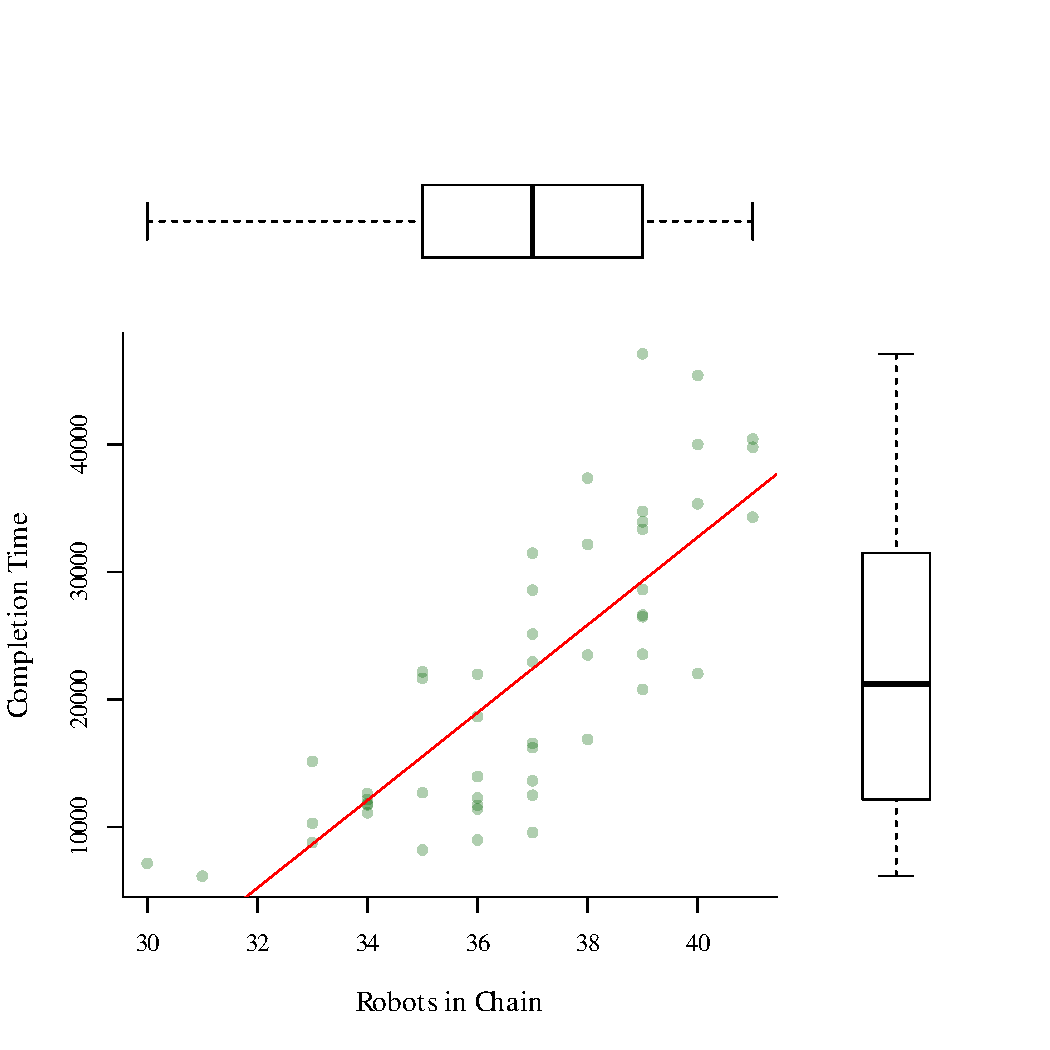
\includegraphics[width=\textwidth,keepaspectratio]{{../Results/50Trials/ResultsDistribution}.pdf}

(a)

\end{center}
\end{minipage}%
\hspace{0.5cm}
\begin{minipage}{.35\textwidth}
\begin{footnotesize}
\begin{center}

\begin{tabular}{|l|c|c|}
\hline
& \textbf{Value} & \textbf{P-Value} \\
\hline
\textbf{Pearson - } $\mathbf{r}$  &	0.7934599 & 6.357e-12 \\
\hline
\textbf{Kendall -} $\mathbf{\tau}$ & 0.6691023 & 5.554e-11 \\
\hline
\end{tabular}
\label{tab:correlation}
\vskip15pt
(b)
\vskip15pt

\end{center}
\end{footnotesize}
\end{minipage}
\captionof{figure}{Enhanced scatter plot of the completion times as a function of the number of robots (a), with the results of the correlation analysis (b)}
\end{center}

Intuitively, one may assume that the completion time is positively correlated with respect to the number of robots in chain (since more robots require more time to be deployed).

This intuition is confirmed by the graphical representation of the completion time as a function of the number of robots in the chain, along with the representation of a linear model fitting the points obtained through the experiment as well as by the values of the correlation coefficients, and their statistical significance (attested by a p-value considerably small than the confidence level $1-\alpha=0.05$.

\bibliographystyle{plainnat}
\bibliography{References}



\section{Conclusions}
To summarize the results from the previous analysis:
\begin{itemize}
    \item On this set of instances, the Simulated Annealing algorithm performs generally better than Ant Colony Optimization.
   \item Simulated Annealing is able to generate an higher percentage of feasible and high quality solutions. 
  \item I believe that the strong limitation of computation times, with respect to VND, has a strong impact on the performance of the algorithms as the generally low probability of finding high quality solutions shows, for ACO in particular.
  \item Further improvement on the ACO algorithm could be made by implementing the original \maxmin system and using an heuristic which could make a better use of the locally available information and guide the algorithm towards feasible solutions.
  \item While the performances of the ACO system are comparable, if not slightly worse than the best VND algorithm implemented in the previous implementation exercise, SA has considerably low run-times required to find high-quality solution and higher percentages of feasible solutions, thus outperforming both the aforementioned algorithms.
  \item The usage of average statistics as metrics to measure the quality of the algorithms is strongly biased by the presence of outliers (penalization, in this case).
\end{itemize}



\bibliographystyle{plain}
\bibliography{References}

\end{document}
